\documentclass[12pt,dvipdfmx]{beamer}
\usepackage{graphicx}
\DeclareGraphicsExtensions{.pdf}
\DeclareGraphicsExtensions{.eps}
\graphicspath{{out/}{out/tex/}{out/tex/gpl/}{out/tex/svg/}{out/tex/dot/}}
% \graphicspath{{out/}{out/tex/}{out/pdf/}{out/eps/}{out/tex/gpl/}{out/tex/svg/}{out/pdf/dot/}{out/pdf/gpl/}{out/pdf/img/}{out/pdf/odg/}{out/pdf/svg/}{out/eps/dot/}{out/eps/gpl/}{out/eps/img/}{out/eps/odg/}{out/eps/svg/}}
\usepackage{listings}
\usepackage{fancybox}
\usepackage{hyperref}
\usepackage{color}

%%%%%%%%%%%%%%%%%%%%%%%%%%%
%%% themes
%%%%%%%%%%%%%%%%%%%%%%%%%%%
\usetheme{Szeged} 
%% no navigation bar
% default boxes Bergen Boadilla Madrid Pittsburgh Rochester
%% tree-like navigation bar
% Antibes JuanLesPins Montpellier
%% toc sidebar
% Berkeley PaloAlto Goettingen Marburg Hannover Berlin Ilmenau Dresden Darmstadt Frankfurt Singapore Szeged
%% Section and Subsection Tables
% Copenhagen Luebeck Malmoe Warsaw

%%%%%%%%%%%%%%%%%%%%%%%%%%%
%%% innerthemes
%%%%%%%%%%%%%%%%%%%%%%%%%%%
% \useinnertheme{circles}	% default circles rectangles rounded inmargin

%%%%%%%%%%%%%%%%%%%%%%%%%%%
%%% outerthemes
%%%%%%%%%%%%%%%%%%%%%%%%%%%
% outertheme
% \useoutertheme{default}	% default infolines miniframes smoothbars sidebar sprit shadow tree smoothtree


%%%%%%%%%%%%%%%%%%%%%%%%%%%
%%% colorthemes
%%%%%%%%%%%%%%%%%%%%%%%%%%%
\usecolortheme{seahorse}
%% special purpose
% default structure sidebartab 
%% complete 
% albatross beetle crane dove fly seagull 
%% inner
% lily orchid rose
%% outer
% whale seahorse dolphin

%%%%%%%%%%%%%%%%%%%%%%%%%%%
%%% fontthemes
%%%%%%%%%%%%%%%%%%%%%%%%%%%
\usefonttheme{serif}  
% default professionalfonts serif structurebold structureitalicserif structuresmallcapsserif

%%%%%%%%%%%%%%%%%%%%%%%%%%%
%%% generally useful beamer settings
%%%%%%%%%%%%%%%%%%%%%%%%%%%
% 
\AtBeginDvi{\special{pdf:tounicode EUC-UCS2}}
% do not show navigation
\setbeamertemplate{navigation symbols}{}
% show page numbers
\setbeamertemplate{footline}[frame number]

%%%%%%%%%%%%%%%%%%%%%%%%%%%
%%% define some colors for convenience
%%%%%%%%%%%%%%%%%%%%%%%%%%%

\newcommand{\mido}[1]{{\color{green}#1}}
\newcommand{\mura}[1]{{\color{purple}#1}}
\newcommand{\ore}[1]{{\color{orange}#1}}
\newcommand{\ao}[1]{{\color{blue}#1}}
\newcommand{\aka}[1]{{\color{red}#1}}

\setbeamercolor{ex}{bg=cyan!20!white}

%%%%%%%%%%%%%%%%%%%%%%%%%%%
%%% how to typset code
%%%%%%%%%%%%%%%%%%%%%%%%%%%

\lstset{language = C,
numbers = left,
numberstyle = {\tiny \emph},
numbersep = 10pt,
breaklines = true,
breakindent = 40pt,
frame = tlRB,
frameround = ffft,
framesep = 3pt,
rulesep = 1pt,
rulecolor = {\color{blue}},
rulesepcolor = {\color{blue}},
flexiblecolumns = true,
keepspaces = true,
basicstyle = \ttfamily\scriptsize,
identifierstyle = ,
commentstyle = ,
stringstyle = ,
showstringspaces = false,
tabsize = 4,
escapechar=\@,
}

\title{Shell and Emacs \\
with little customizations }
\institute{}
\author{田浦}
\date{}

\AtBeginSubsection[] % Do nothing for \section*
{
\begin{frame}
\frametitle{Contents}
\tableofcontents[currentsection,currentsubsection]
\end{frame}
}

\begin{document}
\maketitle

%%%%%%%%%%%%%%%%% 
\begin{frame}
\frametitle{すべての目的}
\begin{itemize}
\item 作業のピークスピードの向上

\item 知っとけば作業効率がぐんとあがること

\item だが,意外と使われていない(知られていない)と感じること

  \begin{itemize}
  \item 入力の削減
  \item マウスを使わない,遠いキー(e.g., 矢印キー)を使わない,
    長距離を一気に移動する,etc.
  \end{itemize}

\item 注: ここでは,「カスタマイズしまくってめっちゃ
  便利に」みたいなことをして,人を引かせるようなことは
  \aka{しません}

% \item 「アホとハサミをどう使うか」という話
\end{itemize}
\end{frame}

%%%%%%%%%%%%%%%%% 
\begin{frame}[fragile]
\frametitle{以降すべての前提}

\begin{itemize}
\item まずはctrlキーを「正しい」位置に直す!
\begin{lstlisting}
$ gnome-tweak-tool    
\end{lstlisting}%$
\end{itemize}
タイピング$\rightarrow$Ctrlキーの位置
\end{frame}


%%%%%%%%%%%%%%%%% 
\begin{frame}
\frametitle{始める前に\ldots}
日本国憲法第20条

\begin{quote}
\begin{itemize}
\item \aka{信教の自由は、何人に対してもこれを保障する。}
いかなる宗教団体も、国から特権を受け、又は政治上の権力を行使してはならない。
\item 何人も、宗教上の行為、祝典、儀式又は行事に参加することを強制されない。
\item 
\aka{国及びその機関は、宗教教育その他いかなる宗教的活動もしてはならない。}
\end{itemize}
\end{quote}

日本国憲法第21条

\begin{quote}
集会、結社及び言論、出版その他一切の表現の自由は、これを保障する。
(以下略)
\end{quote}

\end{frame}
      

%%%%%%%%%%%%%%%%% 
\begin{frame}
\frametitle{補完 (シェル, Emacs共通)}
2,3文字に一回は {\huge タブ} を打とう

\begin{itemize}
\item タイプ時間の節約
\item \aka{タイプミスの削減}
\end{itemize}
\end{frame}

%%%%%%%%%%%%%%%%% 
\begin{frame}[fragile]
\frametitle{シェル: ヒストリ}
\begin{itemize}
\item \ao{上矢印} (最近入れたコマンドを引き出す)
\item \texttt{\ao{C-r}} ... (... に入れた文字列を含むコマンドを引き出す)
\item どちらも,引き出したあとで\ao{編集可能}
\begin{lstlisting}
CFLAGS="-O0 -g" ./configure --prefix=$HOME/install/gnuplot
\end{lstlisting}%$
なんて打つのは一日一回でたくさん!

\item シェルのコマンドライン編集のキー操作は,Emacsと共通
(C-a, C-eなど)

\end{itemize}
\end{frame}

%%%%%%%%%%%%%%%%% 
\begin{frame}[fragile]
\frametitle{知らなきゃダメよ〜,ダメダメ,なコマンド}
\begin{itemize}
\item \aka{lv} : 
スクロールしながら長いファイルを表示; \aka{\texttt{/}} で検索;
.gzなどは勝手にほどいてくれる
\item \aka{grep} : 検索; \aka{\texttt -r}でディレクトリを再帰検索; 
\aka{\texttt -I}はバイナリファイルを無視; e.g.,
\begin{lstlisting}
grep -rI typedef .
\end{lstlisting}
\end{itemize}

\begin{columns}
  \begin{column}{0.75\textwidth}
\begin{itemize}
\item \aka{find} : 種々の条件でファイルを検索; e.g., 
\begin{lstlisting}
find . -name malloc.c
\end{lstlisting}
\item \aka{locate} : システム全体でファイル名を探す; e.g.,
\begin{lstlisting}
locate *libgtk*.so
\end{lstlisting}
\end{itemize}
\end{column}

\begin{column}{0.25\textwidth}
\includegraphics[width=\textwidth]{out/pdf/svg/dameyo.pdf}
\end{column}
\end{columns}
\end{frame}

%%%%%%%%%%%%%%%%% 
\begin{frame}
  \begin{columns}
    \begin{column}{0.5\textwidth}
{\huge これから「Emacs」の話をしよう}
\vskip1cm
{\large いまを生き延びるためのエディタ}
    \end{column}
    \begin{column}{0.5\textwidth}
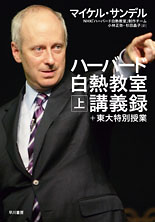
\includegraphics[height=0.9\textheight]{out/pdf/img/sandel.pdf}
    \end{column}
  \end{columns}
  \begin{center}
  \end{center}

\end{frame}

%%%%%%%%%%%%%%%%% 
\begin{frame}
\frametitle{Emacs: カーソル移動の小技}
少し覚えれば確実に少し便利になるいくつかのキー

\begin{itemize}
\item \texttt{\ao{C-a}} (行頭)と \texttt{\ao{C-e}} (行末)
\item バッファの終わり (\texttt{\ao{M->}}) 
(同じことだが \texttt{\ao{C-[}}をおしてから\texttt{\ao{>}})
\end{itemize}

なるべく,矢印キーを押して「つつつつつつ\ldots 」
をやらないことを心がける

\end{frame}

%%%%%%%%%%%%%%%%% 
\begin{frame}
\frametitle{小脱線: メタキーの色々なうち方}
\ao{\texttt{M-}} と言われたら,以下のどれでも良い

\begin{itemize}
\item<2-> Alt を\aka{押しながら}
\item<3-> ESC を\ao{押してから}
\item<4-> {\LARGE\ao{\tt C-[} を押してから}
  \only<5->{$\leftarrow$ 実はこれがオススメ}
\end{itemize}

\only<6->{理由:}

\begin{itemize}
\item<7-> Altは手を動かす必要が生じる; 「押しながら」は辛いときがある(e.g., Alt $+$ シフト $+ \cdots$).
キーボードによってはどれがそれなのかわからないことも
\item<8-> ESCは遠い.xとも遠い (\ao{\texttt{M-x}})
\item<9-> そいつらは他の目的に奪われたりしがち
\item<10-> \texttt{\ao{C-[}}は安定している
\item<11-> {\footnotesize もちろんCtrlキーは正しい位置にあることが前提}
\end{itemize}
\end{frame}



%%%%%%%%%%%%%%%%% 
\begin{frame}
\frametitle{Emacs: \texttt{\ao{C-s}} と \texttt{\ao{C-r}}}

\begin{itemize}
\item 「\texttt{\ao{C-s}} 文字列」 で文字列前方インクリメンタル検索
\item 「\texttt{\ao{C-r}} 文字列」 で文字列後方インクリメンタル検索

\item 同じ文字列で次を検索したければ,
\texttt{\ao{C-s}} (または\texttt{\ao{C-r}}) 
  を連打
\item<2-> {\footnotesize もちろんCtrlキーは正しい位置にあることが前提}
\end{itemize}
\end{frame}

%%%%%%%%%%%%%%%%% 
\begin{frame}
\frametitle{Emacs: \texttt{\ao{C-s}}
  は他のエディタの検索とは違うのだよ!}
\begin{itemize}
\item \aka{一瞬で}検索を初められ,
\item 一文字打つごとにそこまでの文字が検索され,
\item 見つかったところですぐにやめればいい.
\end{itemize}

\begin{center}

\includegraphics[width=0.5\textwidth]{out/pdf/img/zaku.pdf}
\end{center}
\end{frame}

%%%%%%%%%%%%%%%%% 
\begin{frame}
\frametitle{Emacs: \texttt{\ao{C-s}}
  は他のエディタの検索とは違うのだよ!}
\begin{itemize}
\item (英語の文章やプログラムならば)
  ほとんど「カーソル移動」の手段と言ってもいいくらい
\item \ao{カーソル移動は以下で:}
  \begin{itemize}
  \item \texttt{C-a} (行頭), \texttt{C-e} (行末)
  \item \aka{\texttt{C-s} (前方), \texttt{C-r} (後方)}
  \item \texttt{C-f} (右), \texttt{C-b} (左), \texttt{C-p} (上), \texttt{C-n} (下)
  \end{itemize}
\end{itemize}
\end{frame}


%%%%%%%%%%%%%%%%% 
\begin{frame}
\frametitle{Emacs: マウスなしのコピペを使いこなそう}

\begin{itemize}
\item 選びたい領域の,
  \begin{itemize}
  \item 端っこで \texttt{\ao{C-SPACE}} (もしかすると \texttt{\ao{C-@}};
    ``Mark set'')
  \item もうひとつの端っこへカーソル移動
  \end{itemize}
\item その状態で
  \begin{itemize}
  \item cut: \texttt{\ao{C-w}}
  \item paste: \texttt{\ao{C-y}}
  \end{itemize}
\item ちなみに,
  \begin{itemize}
  \item copy: \texttt{\ao{M-w}} (つまり \texttt{\ao{C-[ w}})
  \item 別途覚える必要はあまりないという説もある
    \texttt{\ao{M-w}} $\approx$ \texttt{\ao{C-w}} ; \texttt{\ao{C-y}}
  \item 用途: 編集不可のファイルか
  \item 用途: 一瞬でも消すのがためらわれる大きな領域
  \end{itemize}
\end{itemize}
\end{frame}


%%%%%%%%%%%%%%%%% 
\begin{frame}[fragile]
\frametitle{Emacs: マウスなしのコピペを使いこなそう}
\texttt{\ao{C-k}}が1〜数行のcut-pasteに有用 
\begin{itemize}
\item 今いる場所からその行末(の直前)までをcut : \texttt{\ao{C-k}}
\item 直後にもう一度 \texttt{\ao{C-k}} で行末も cut
\item さらに繰り返せば 2行3行\ldots とまとめてcut
\item \texttt{\ao{C-a}} (行頭へジャンプ)と組み合わせて使いこなそう
\item 使用例: 
  \begin{itemize}
  \item 1行まるごと cut 
\begin{lstlisting}
C-a C-k C-k
\end{lstlisting}
\item 1行まるごと複製
\begin{lstlisting}
C-a C-k C-k C-y C-y
\end{lstlisting}
\item 3行まるごと複製
\begin{lstlisting}
C-a C-k@$\times 6$@ C-y C-y
\end{lstlisting}
  \end{itemize}
\end{itemize}
\end{frame}

%%%%%%%%%%%%%%%%% 
\begin{frame}[fragile]
\frametitle{コピペ応用編}
関数をいっこ,まるごと複製する(いじる前によくやるやつ)
\begin{lstlisting}
generic *
gp_alloc(size_t size, const char *message)
{
    char *p;			/* the new allocation */

>       ...

    return (p);
}
\end{lstlisting}

\begin{itemize}
\item 関数先頭へ移動 (検索で! \texttt{\ao{C-r generic}})
\item マークを残す (\texttt{\ao{C-SPACE}})
\item 関数終りへ移動 (検索で! \texttt{\ao{C-s ...}})
\item cut;paste;paste; (\texttt{\ao{C-w C-y C-y}})
\end{itemize}
\end{frame}




%%%%%%%%%%%%%%%%% 
\begin{frame}
\frametitle{Emacs: M-x shellのススメ}
\begin{itemize}
\item Emacsの中でシェルを立ち上げる
\item 何が便利? 色々
  \begin{itemize}
  \item やったことを保存してくれる(configureで何か怒られてなかった???)
  \item 結果をコピペ(日記に書く)
  \item 前のコマンドの再入力(コマンド行に戻ってENTERでOK)
  \item シェルとの間で行き来の手間が減る
  \end{itemize}
\item その他,Emacsの中で生活することのすすめ
  (M-x grep, gud-gdb, compile, etc.)
\item ファイルを編集するたびに立ち上げなおすものではない
\end{itemize}
\end{frame}




%%%%%%%%%%%%%%%%% 
\begin{frame}[fragile]
\frametitle{Emacs: C-r と M-x shell}
\begin{itemize}
\item 例1: Emacsのシェル内で過去に入力したコマンドを探して再入力
  $\Rightarrow$
\begin{lstlisting}
C-r プロンプトの文字列 C-r C-r C-r ...
\end{lstlisting} %$
\item 例2: configure で何かwarningなかった?? $\Rightarrow$
\begin{lstlisting}
 C-r warning:
\end{lstlisting}
\item 例2: \aka{最後の}configure で何かwarningなかった?? $\Rightarrow$
  \begin{itemize}
  \item C-r で一旦最後のコマンドの入力行へ戻り
  \item C-s warning で前方に検索
  \end{itemize}
\end{itemize} %$
\end{frame}


%%%%%%%%%%%%%%%%% 
\begin{frame}[fragile]
\frametitle{置換}
\begin{itemize}
\item M-x query-replace (一個ずつ確認しながら置換)
\item M-x replace-string (一気に置換)
\item キーボードマクロ (これまでに学んだわざと組み合わせて,汎用,強力,
  かつお手軽な自動化手法)
\end{itemize}
\end{frame}


%%%%%%%%%%%%%%%%% 
\begin{frame}
\frametitle{キーボードマクロ}
\begin{itemize}
\item \ao{\texttt{C-x (}} : 記録開始
\item \ao{\texttt{C-x )}} : 記録終了
\item \ao{\texttt{C-x e}} : 記録内容実行
\item 回数のバリエーション
  \begin{itemize}
  \item \texttt{C-u C-x e} : 記録内容を4回実行
  \item \texttt{C-u C-u C-x e} : 記録内容を16 ($= 4^2$)回実行
  \item \texttt{C-u C-u C-u C-x e} : 記録内容を64 ($= 4^3$)回実行
  \item \texttt{C-u $n$ C-x e} : 記録内容を$n$回実行
  \end{itemize}
\end{itemize}
\end{frame}

%%%%%%%%%%%%%%%%% 
\begin{frame}
\frametitle{キーボードマクロを使う上での要点}
\begin{itemize}
\item ある意味を持った一連の編集作業が,「全く同じキー操作」でできるようにする
\item そのために,これまでの技\texttt{C-a, C-e, C-s}などが有効
\item 「一文字移動」だけでは単語の長さの違いなどを吸収できない
\end{itemize}


\end{frame}


%%%%%%%%%%%%%%%%% 
\begin{frame}
\frametitle{Emacs: 知っとかないといらつく編}
\begin{itemize}
\item ここまでは,「オフェンス」
\item 以下は「ディフェンス」
  \begin{itemize}
  \item とりたてて「便利」というわけではなく,
    知っとかないとEmacs嫌いになる項目
  \end{itemize}

\item ひとつ目: コマンドの最中にやめたくなったら\ao{\texttt{C-g}}
\item ふたつ目: Undo は \ao{\texttt{C-\_}}
\end{itemize}


\end{frame}


%%%%%%%%%%%%%%%%% 
\begin{frame}
\frametitle{Emacs: 窓を整理する}
\begin{itemize}
\item コマンド(M-x shell, gdbなど)を使っていると,
  勝手に窓が割れる
\item それを自在に整理できないとストレス貯まる
  \begin{itemize}
  \item \texttt{\ao{C-x 0}} : その窓を非表示にする
  \item \texttt{\ao{C-x 1}} : その窓\aka{だけを表示}する
  \item \texttt{\ao{C-x 2}} : 水平に割る
  \item \texttt{\ao{C-x 3}} : 垂直に割る
  \end{itemize}
\item \texttt{\ao{C-x o}} : 窓間の移動
\item つまり
  \begin{itemize}
  \item 勝手に割られた窓がうっとおしければ\texttt{\ao{C-x 1}}
  \item また表示したくなったら \texttt{\ao{C-x b}} (割りたければ割る)
  \end{itemize}
\end{itemize}
\end{frame}

%%%%%%%%%%%%%%%%% 
\begin{frame}
\frametitle{Emacs: ファイル間の行き来の仕方}

\begin{itemize}
\item \texttt{\ao{C-x b}} (switch to buffer)
\item ファイル名を覚えていればそれを入力
\item ここでもタブ補完!
\item いきなりタブで一覧表示
\item シェルのバッファは,*shell*
\end{itemize}
もうひとつ,
\begin{itemize}
\item \texttt{\ao{C-x C-b}} バッファ(開いているファイル)一覧
\item カーソルで選んで\texttt{\ao{f}}でそのバッファへ移動
\end{itemize}

\end{frame}

%%%%%%%%%%%%%%%%% 
\begin{frame}[fragile]
\frametitle{最後に}

  \begin{itemize}
  \item ここまでEmacsを一切カスタマイズしなくても出来る.
  \item 参考までに,私がやっている,重要なカスタマイズはひとつ(だけ)
    \begin{itemize}
    \item 他のウィンドウに移動するときの\texttt{C-x o}を,
      \texttt{\ao{C-o}}だけに
    \item やり方: 以下を ~/.emacs に記入
    \end{itemize}
\begin{lstlisting}
(define-key global-map "\C-o" 'other-window)
\end{lstlisting}
 \end{itemize}
\end{frame}


\end{document}



